\chapter{Generative modeling meets representation learning}\label{chapter:generative_modeling_and_representation_learning}

This chapter is about models that unite the ideas of both generative modeling and representation learning. These models learn mappings both to and from data, and simultaneously satisfy the goals of both representation learning and generative modeling.

The intuition is that generative models map a simple base distribution (``noise") to data, whereas representation learning maps data to simple underlying representations (``embeddings"). These two problems are, essentially, inverses of each other. Many algorithms explicitly treat them as inverse problems, where solving the problem in one direction can inform the solution in the other direction.

In Chapter \ref{chapter:neural_nets}, we described neural nets as being a sequence of mappings from raw data to ever more abstracted representations, layer by layer. This perspective puts representation learning in the spotlight: deep learning is just representation learning! Let us now point out an alternative perspective: in backwards order, deep nets are mappings from abstracted representations to ever more concrete representations of the data, layer by layer, until at the final layer (the input) we arrive at the raw data itself. This ``backwards" ordering is the direction in which deep generative networks work. This perspective puts the spotlight on generative modeling: deep learning is just generative modeling! Indeed both modeling directions are valid, and the full picture looks like this:\marginnote{Here we label one side as ``Data" and the other as ``Embedding", but what's the precise difference between these two things? Why is an RGB image ``data" while a 100-dimensional vector of neural activations is an ``embedding"? This is a question for you to think about; there is no right answer.}[2cm]
\begin{figure}[h!]
    \centering
    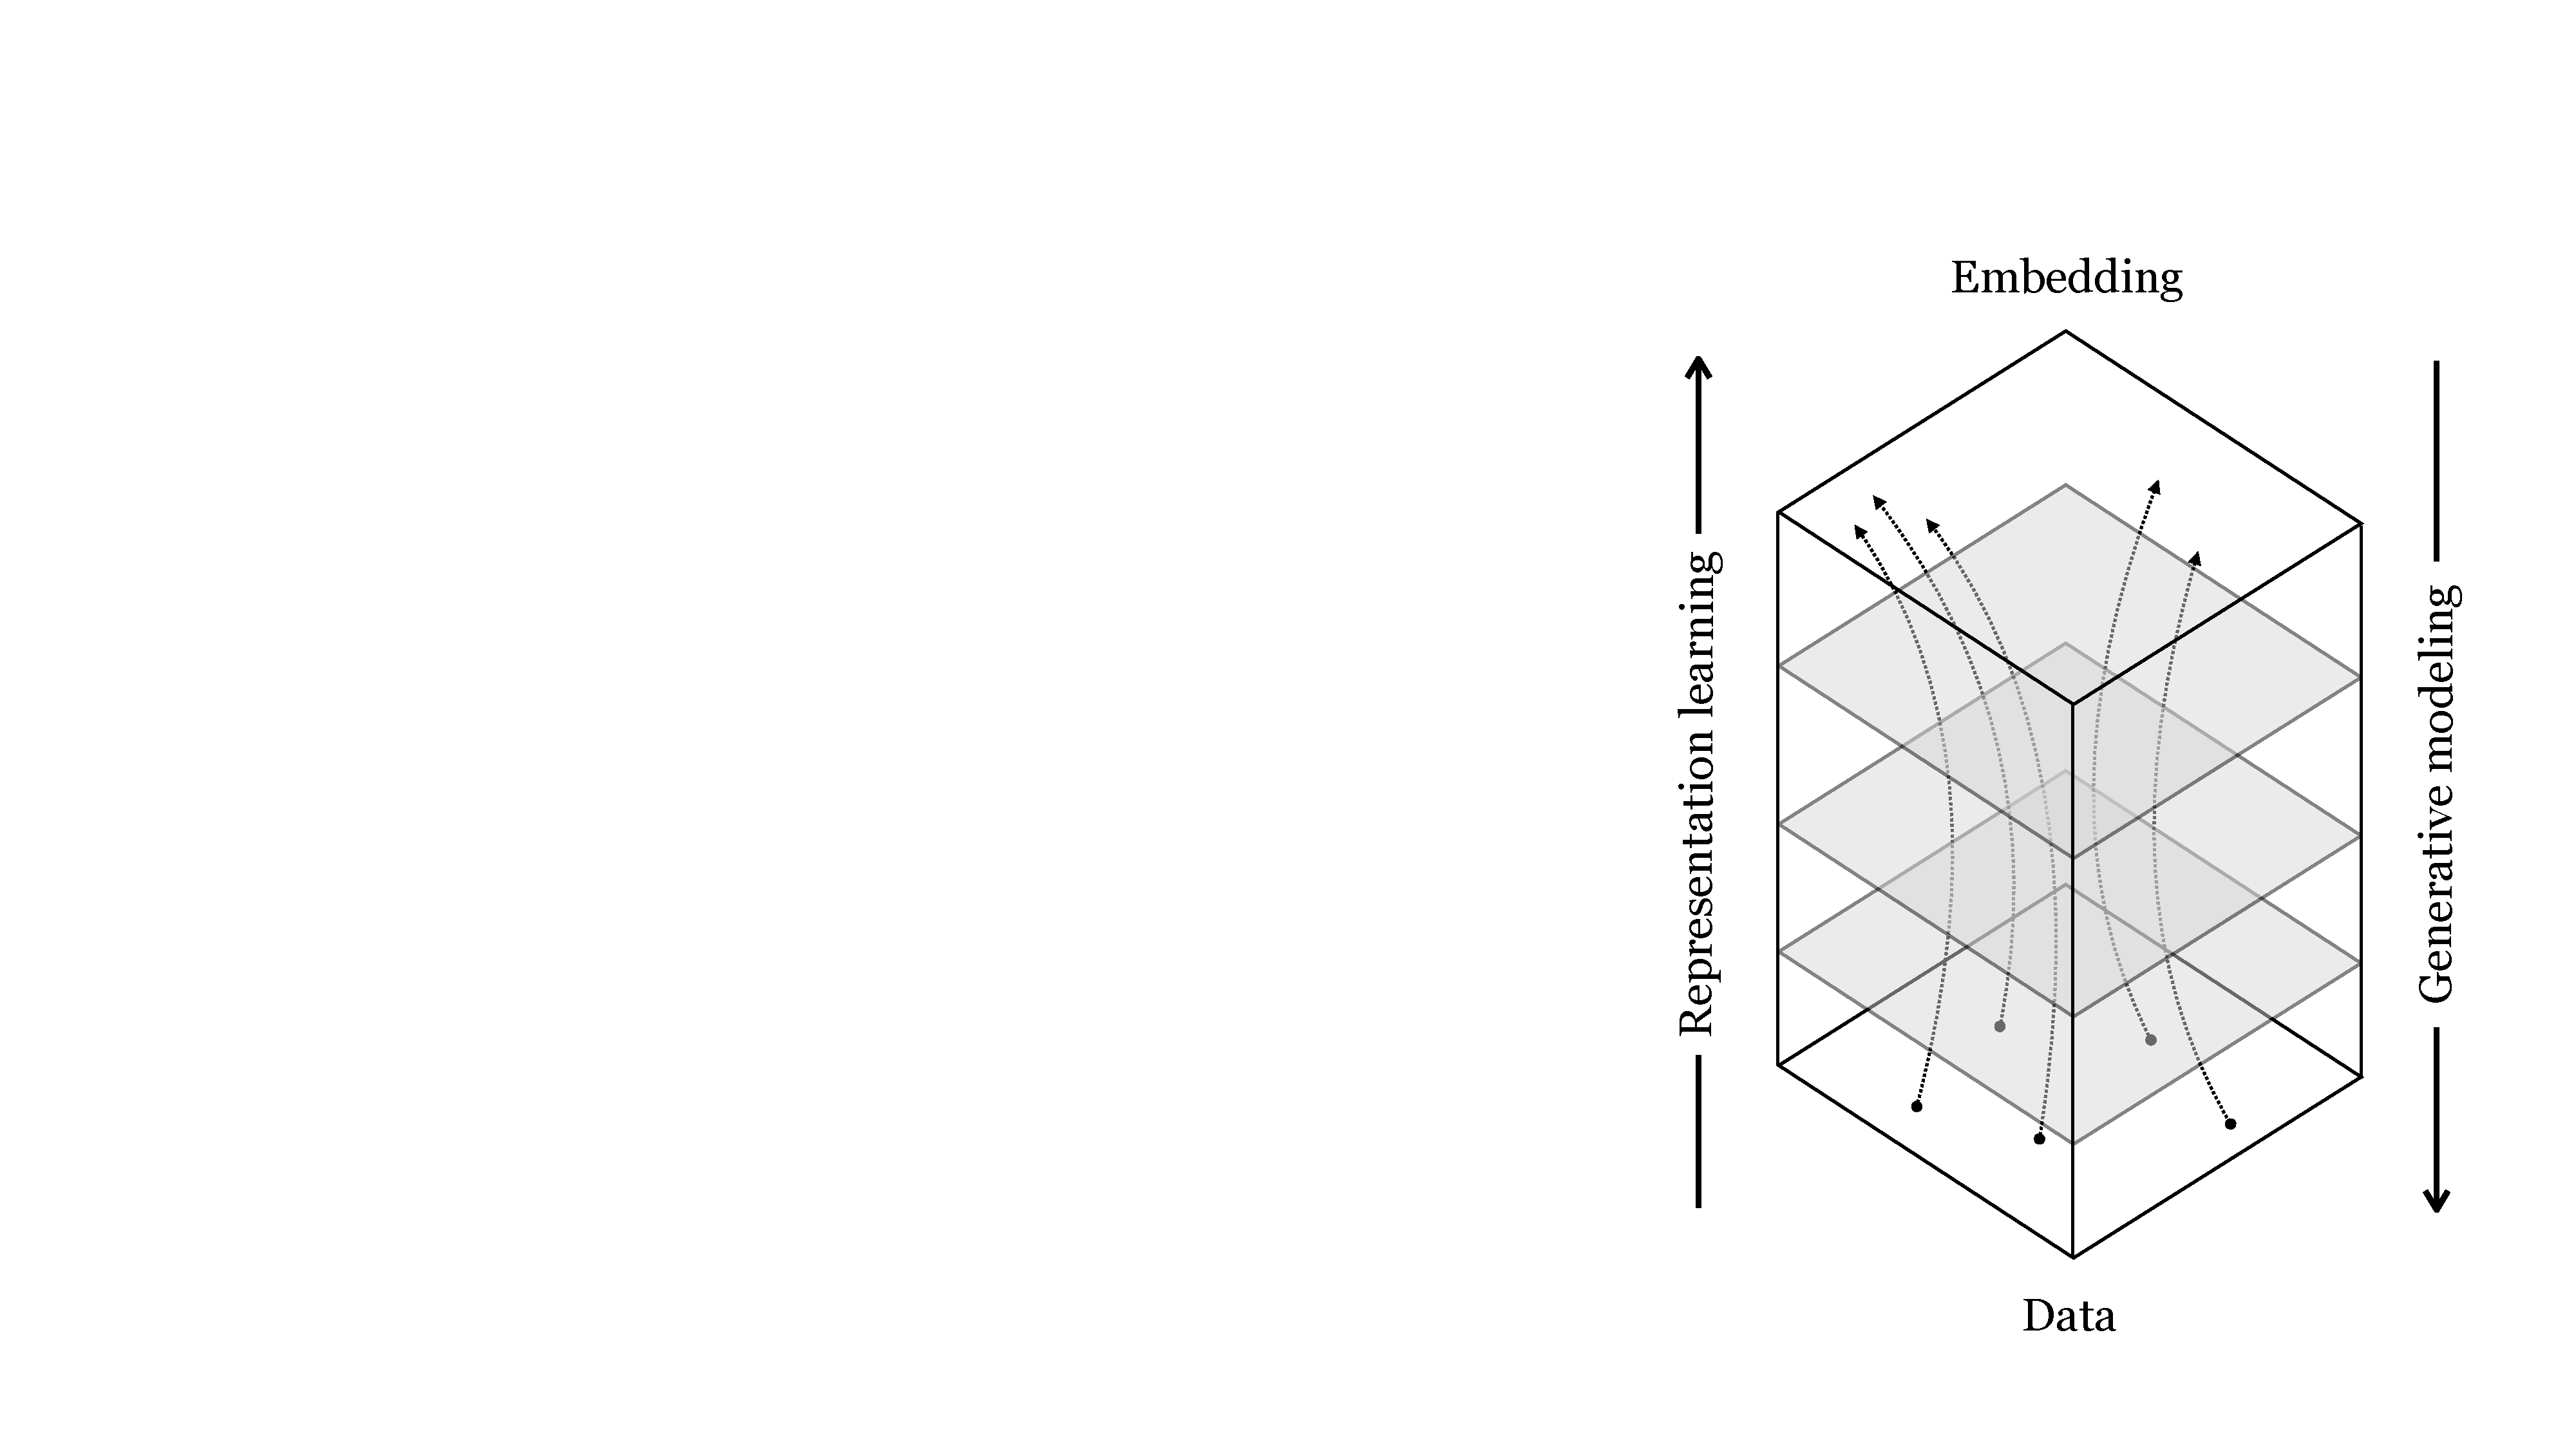
\includegraphics[width=0.4\linewidth]{./figures/generative_modeling_and_representation_learning/rep_gen_schematic.pdf}
    \label{fig:generative_modeling_and_representation_learning:rep_gen_schematic}
\end{figure}

\section{Latent variables as representations}

In Chapter \ref{chapter:generative_models}, we introduced generative models with latent variables $\mathbf{z}$. In that context, the role of the latent variable was to specify all unobserved factors that might affect the output of a model. For example, if the model predicts the color of a black and white photo, it is a mapping $g: \mathbf{x}, \mathbf{z} \rightarrow \mathbf{y}$, with $\mathbf{x}$ being the black and white input, $\mathbf{y}$ being the color output and $\mathbf{z}$ being any other information that needs to be known in order to make the mapping completely deterministic -- for example, the color of a t-shirt which cannot be inferred solely form the black and white input. In the extreme case of unconditional generative models, all properties of the generated images are controlled by the latent variables.

What we did not mention in Chapter \ref{chapter:generative_models}, but will focus on now, is that \textit{latent variables are representations of the data}. In the case of an unconditional generative model, the latent variables are a \textit{complete} representation of the data: all information in the data is represented in the latent variables.

Given this connection, this chapter will ask the question: are latent variables \textit{good} representations of the data? And can they be combined with other representation learning algorithms?

%The main idea is that latent variables are representations. 

%We have already seen representation learning as the problem of mapping data $\mathbf{x}$ to ``embedding" $\mathbf{z}$ and generative modeling as the problem of mapping ``noise" $\mathbf{z}$ to data $\mathbf{x}$. You may have wondered why we used the same variable name, $\mathbf{z}$, for these seemingly different things. The reason is because they are actually highly related! Both embeddings and noise are representations that have a deterministic functional relationship to the data, $\mathbf{z} = E(\mathbf{x})$ and $\mathbf{x} = G(\mathbf{z})$. An encoder $E$ performs the inverse functional role as a generator $G$.\marginnote{All generative models map a stochastic noise source to images, but not all interpret the noise source as latent random variables. For example, autoregressive models are fit without reference to any latent variables, and the noise source is only used during sampling.}[-2cm] The models we will describe in this chapter make the connection between noise and embeddings formally precise.

\section{Technical setting}
We will consider random variables $\mathbf{z}$ and $\mathbf{x}$ related as follows, with $g$ being deterministic generator (a.k.a. decoder) and $f$ being a deterministic encoder:
\begin{align}
    &\mathbf{x} \sim p_{\texttt{data}}(\mathbf{x}) &\mathbf{z} \sim p_{\mathbf{z}}(\mathbf{z}) \\
    &\hat{\mathbf{z}} = f(\mathbf{x}) &\hat{\mathbf{x}} = g(\mathbf{z})
\end{align}
$f$ and $g$ will be trained so that $g \approx f^{-1}$ so that $\hat{\mathbf{x}} \approx \mathbf{x}$ and $\hat{\mathbf{z}} \approx \mathbf{z}$. In Figure \ref{fig:representation_learning:rep_learning_schematic}, we sketched how representation learning maps from a data domain to a simple embedding space. We can now put that diagram side by side with the equivalent diagram for generative modeling. Notice again how they are just the same thing in opposite directions:
\begin{figure}[h!]
    \centering
    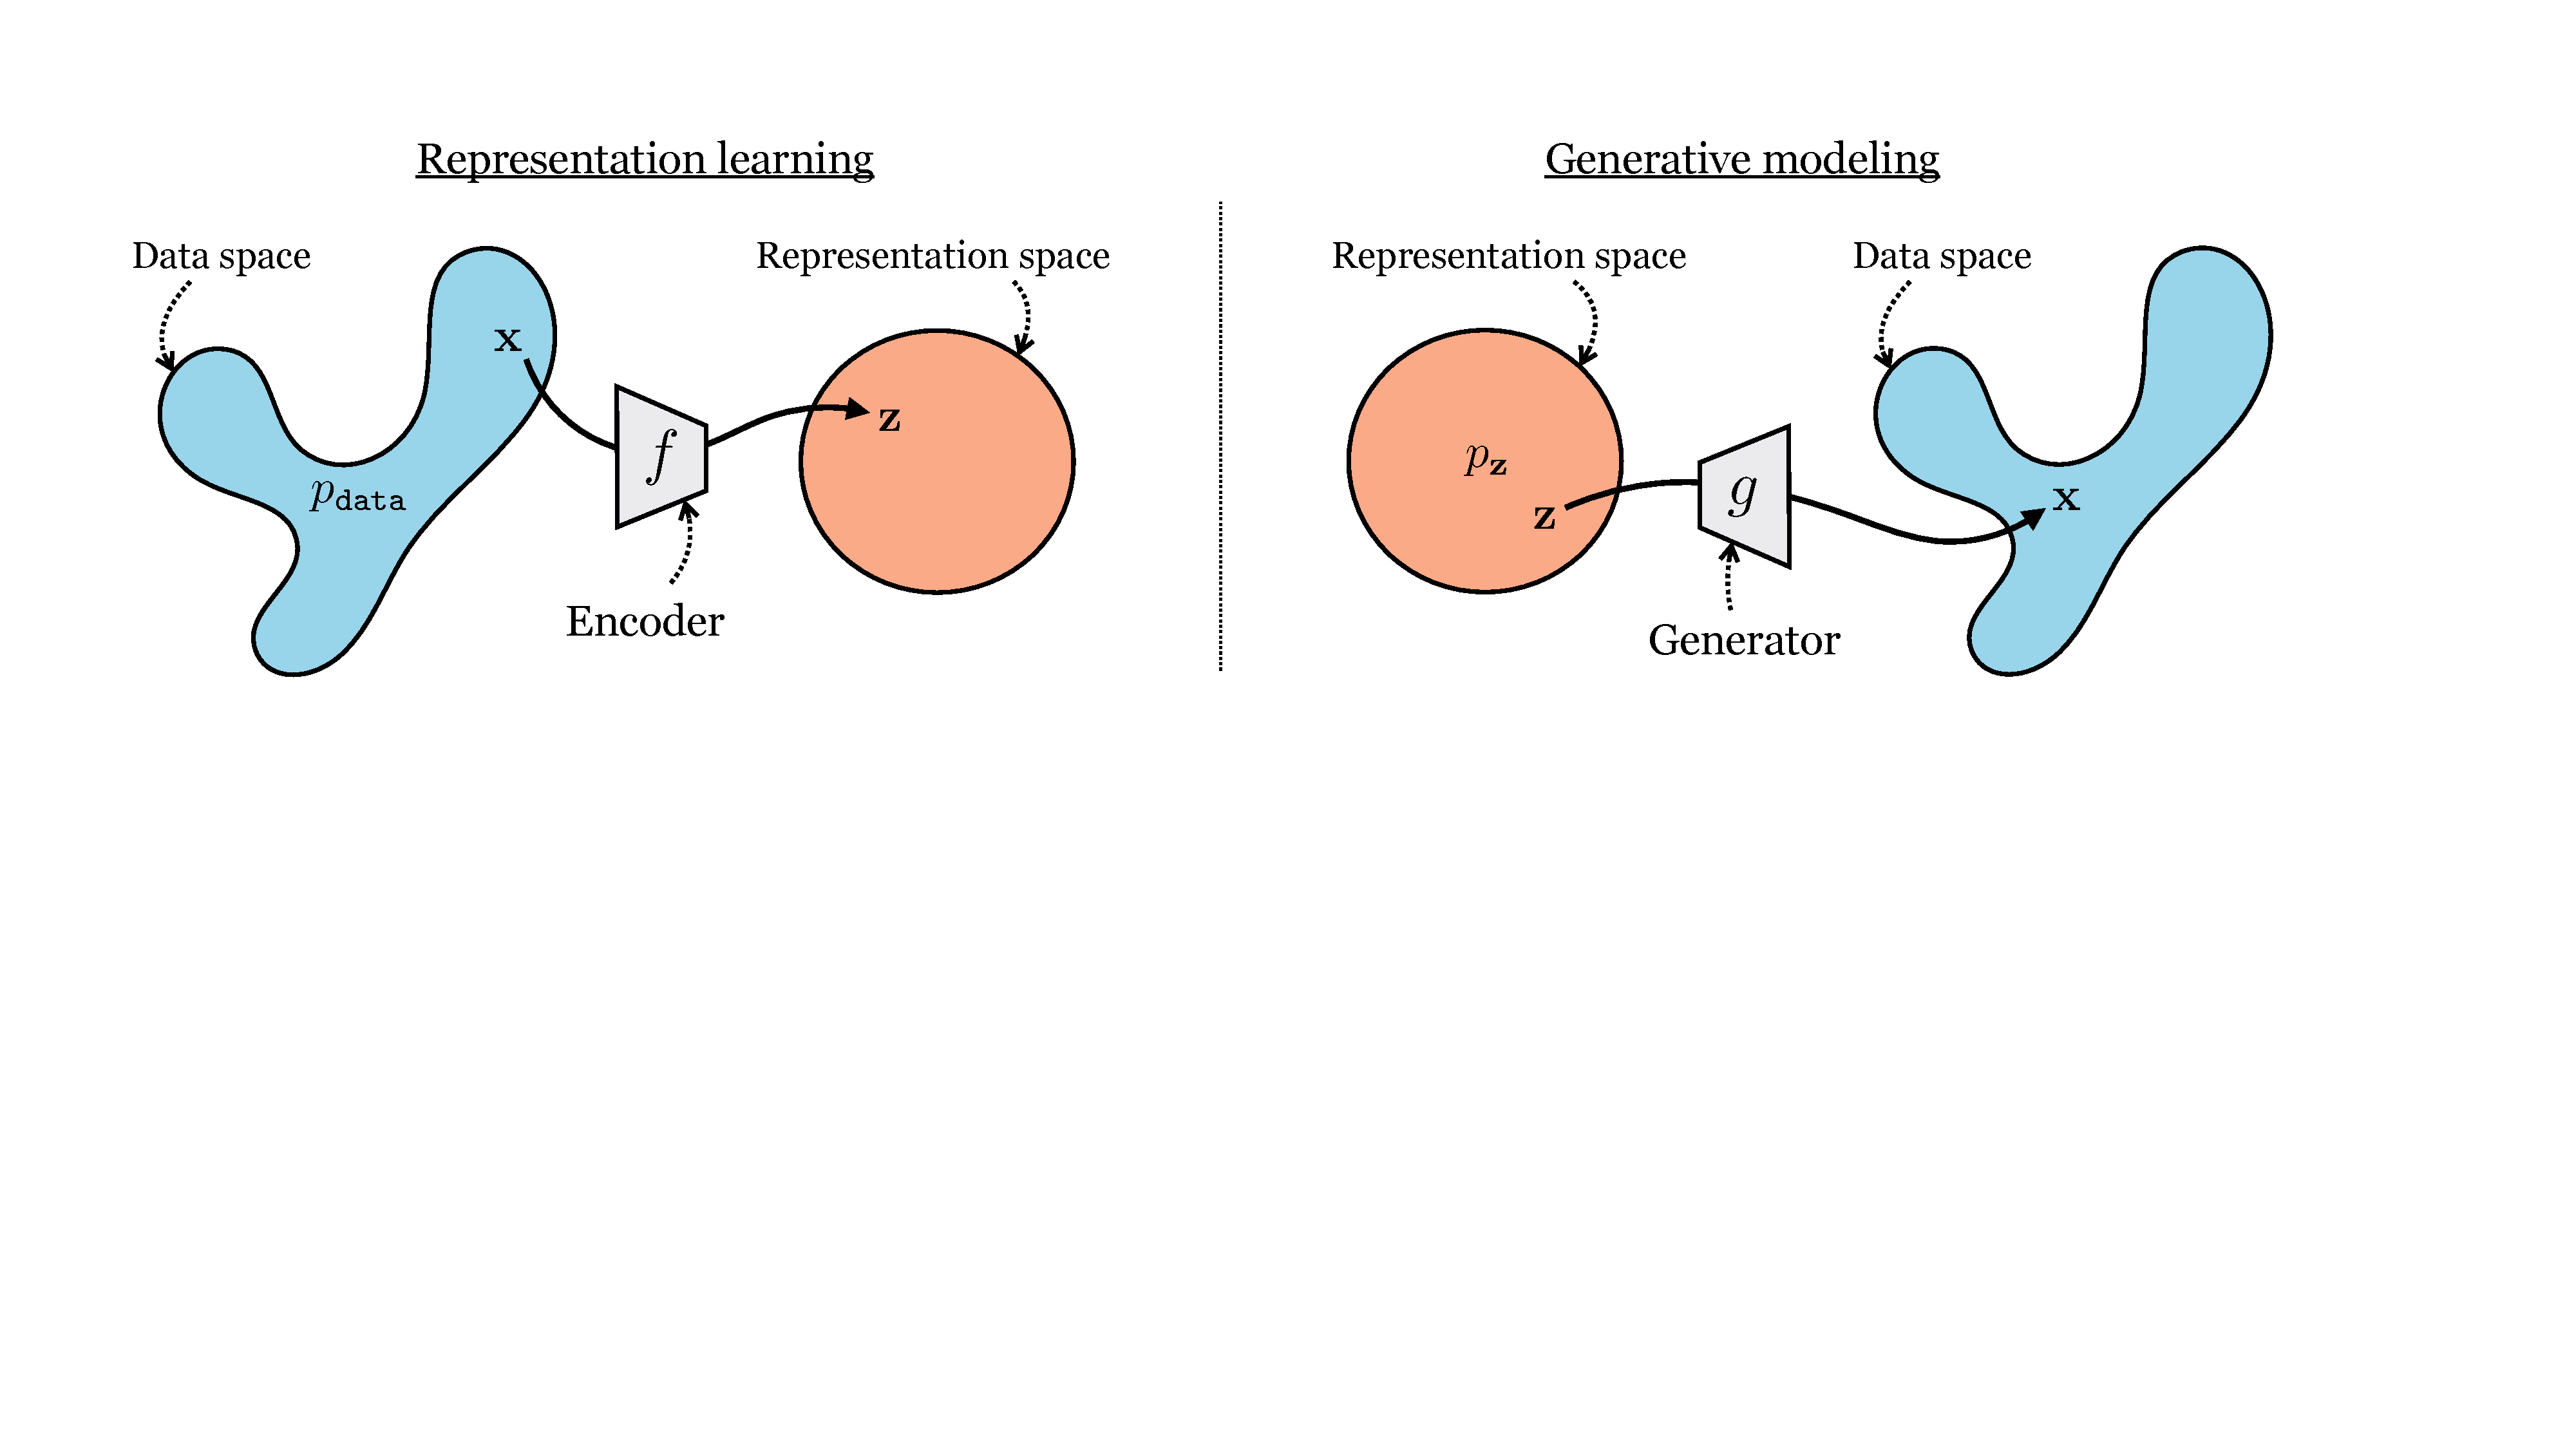
\includegraphics[width=1.0\linewidth]{./figures/generative_modeling_and_representation_learning/genrep_schematic.pdf}
    \caption{Generative modeling performs the opposite mapping from representation learning.}
    \label{fig:generative_modeling_and_representation_learning:genrep_schematic}
\end{figure}

One of the most important quantities we will measure is the data likelihood function $L(\{\mathbf{x}\}_{i=1}^N, \theta)$, which measures the likelihood of the data under the model $p_{\theta}$:
\begin{align}
    L(\{\mathbf{x}^{(i)}\}_{i=1}^N, \theta) = \prod_i p_{\theta}(\mathbf{x}^{(i)})
\end{align}
Many methods use a max likelihood objective, optimizing $L$ w.r.t. $\theta$. To compute the likelihood function, we need to compute $p_{\theta}(\mathbf{x})$. One way to express this function is as the \textbf{marginal likelihood} of $\mathbf{x}$, marginalizing over all unobserved latent variables $\mathbf{z}$:
\begin{align}
    p_{\theta}(\mathbf{x}) = \int_{\mathbf{z}} p_{\theta}(\mathbf{x} | \mathbf{z})p_{\mathbf{z}}(\mathbf{z})d\mathbf{z}\label{eqn:generative_modeling_and_representation_learning:marginal_likelihood_p}
\end{align}
%Here $\mathbf{z}$ are the latent variables. Given an observation $\mathbf{x}$, we may integrate over the latent variables to calculate its probability. 
The advantage of expressing $p_{\theta}(\mathbf{x})$ in this way is that it reduces the modeling problem to learning the conditional distribution $p_{\theta}(\mathbf{x} | \mathbf{z})$, which itself can be straightforwardly modeled using $G$. For example, we could model $p_{\theta}(\mathbf{x} | \mathbf{z}) = \mathcal{N}(\mu = G(\mathbf{z}), \sigma = \mathbf{1})$, i.e . just place a unit Gaussian distribution centered on $G(\mathbf{z})$.

We can also write the marginal likelihood for the probability of a latent vector $\mathbf{z}$ expressed as an integral over $p_{\texttt{data}}$, given a model of the conditional distribution of $\mathbf{z}$ given $\mathbf{x}$:
\begin{align}
    q_{\theta}(\mathbf{x}) = \int_{\mathbf{x}} q_{\theta}(\mathbf{z} | \mathbf{x})p_{\texttt{data}}(\mathbf{x})d\mathbf{x}\label{eqn:generative_modeling_and_representation_learning:marginal_likelihood_q}
\end{align}
Following standard notation, we use $p$ to refer to probability distributions over data and $q$ to refer to probability distributions over latents.

The integrals in Eqn. \ref{eqn:generative_modeling_and_representation_learning:marginal_likelihood_p} and \ref{eqn:generative_modeling_and_representation_learning:marginal_likelihood_q} are expensive so most generative models either approximate the integral or somehow sidestep the need to explicitly calculate it. We will examine a few such strategies next.

\section{Variational Autoencoders}

\subsection{The decoder of an autoencoder is a data generator}
In Chapter \ref{chapter:representation_learning} we learned about autoencoders. These are models that learn an embedding that can be decoded to reconstruct the input data. You may already have noticed that the decoder of an autoencoder looks just like a generator. It is a mapping from a representation of the data, $\mathbf{z}$, back to the data itself, $\mathbf{x}$. Given a $\mathbf{z}$, we can synthesize an image by passing it through the decoder of the autoencoder:
\begin{figure}[h!]
    \centering
    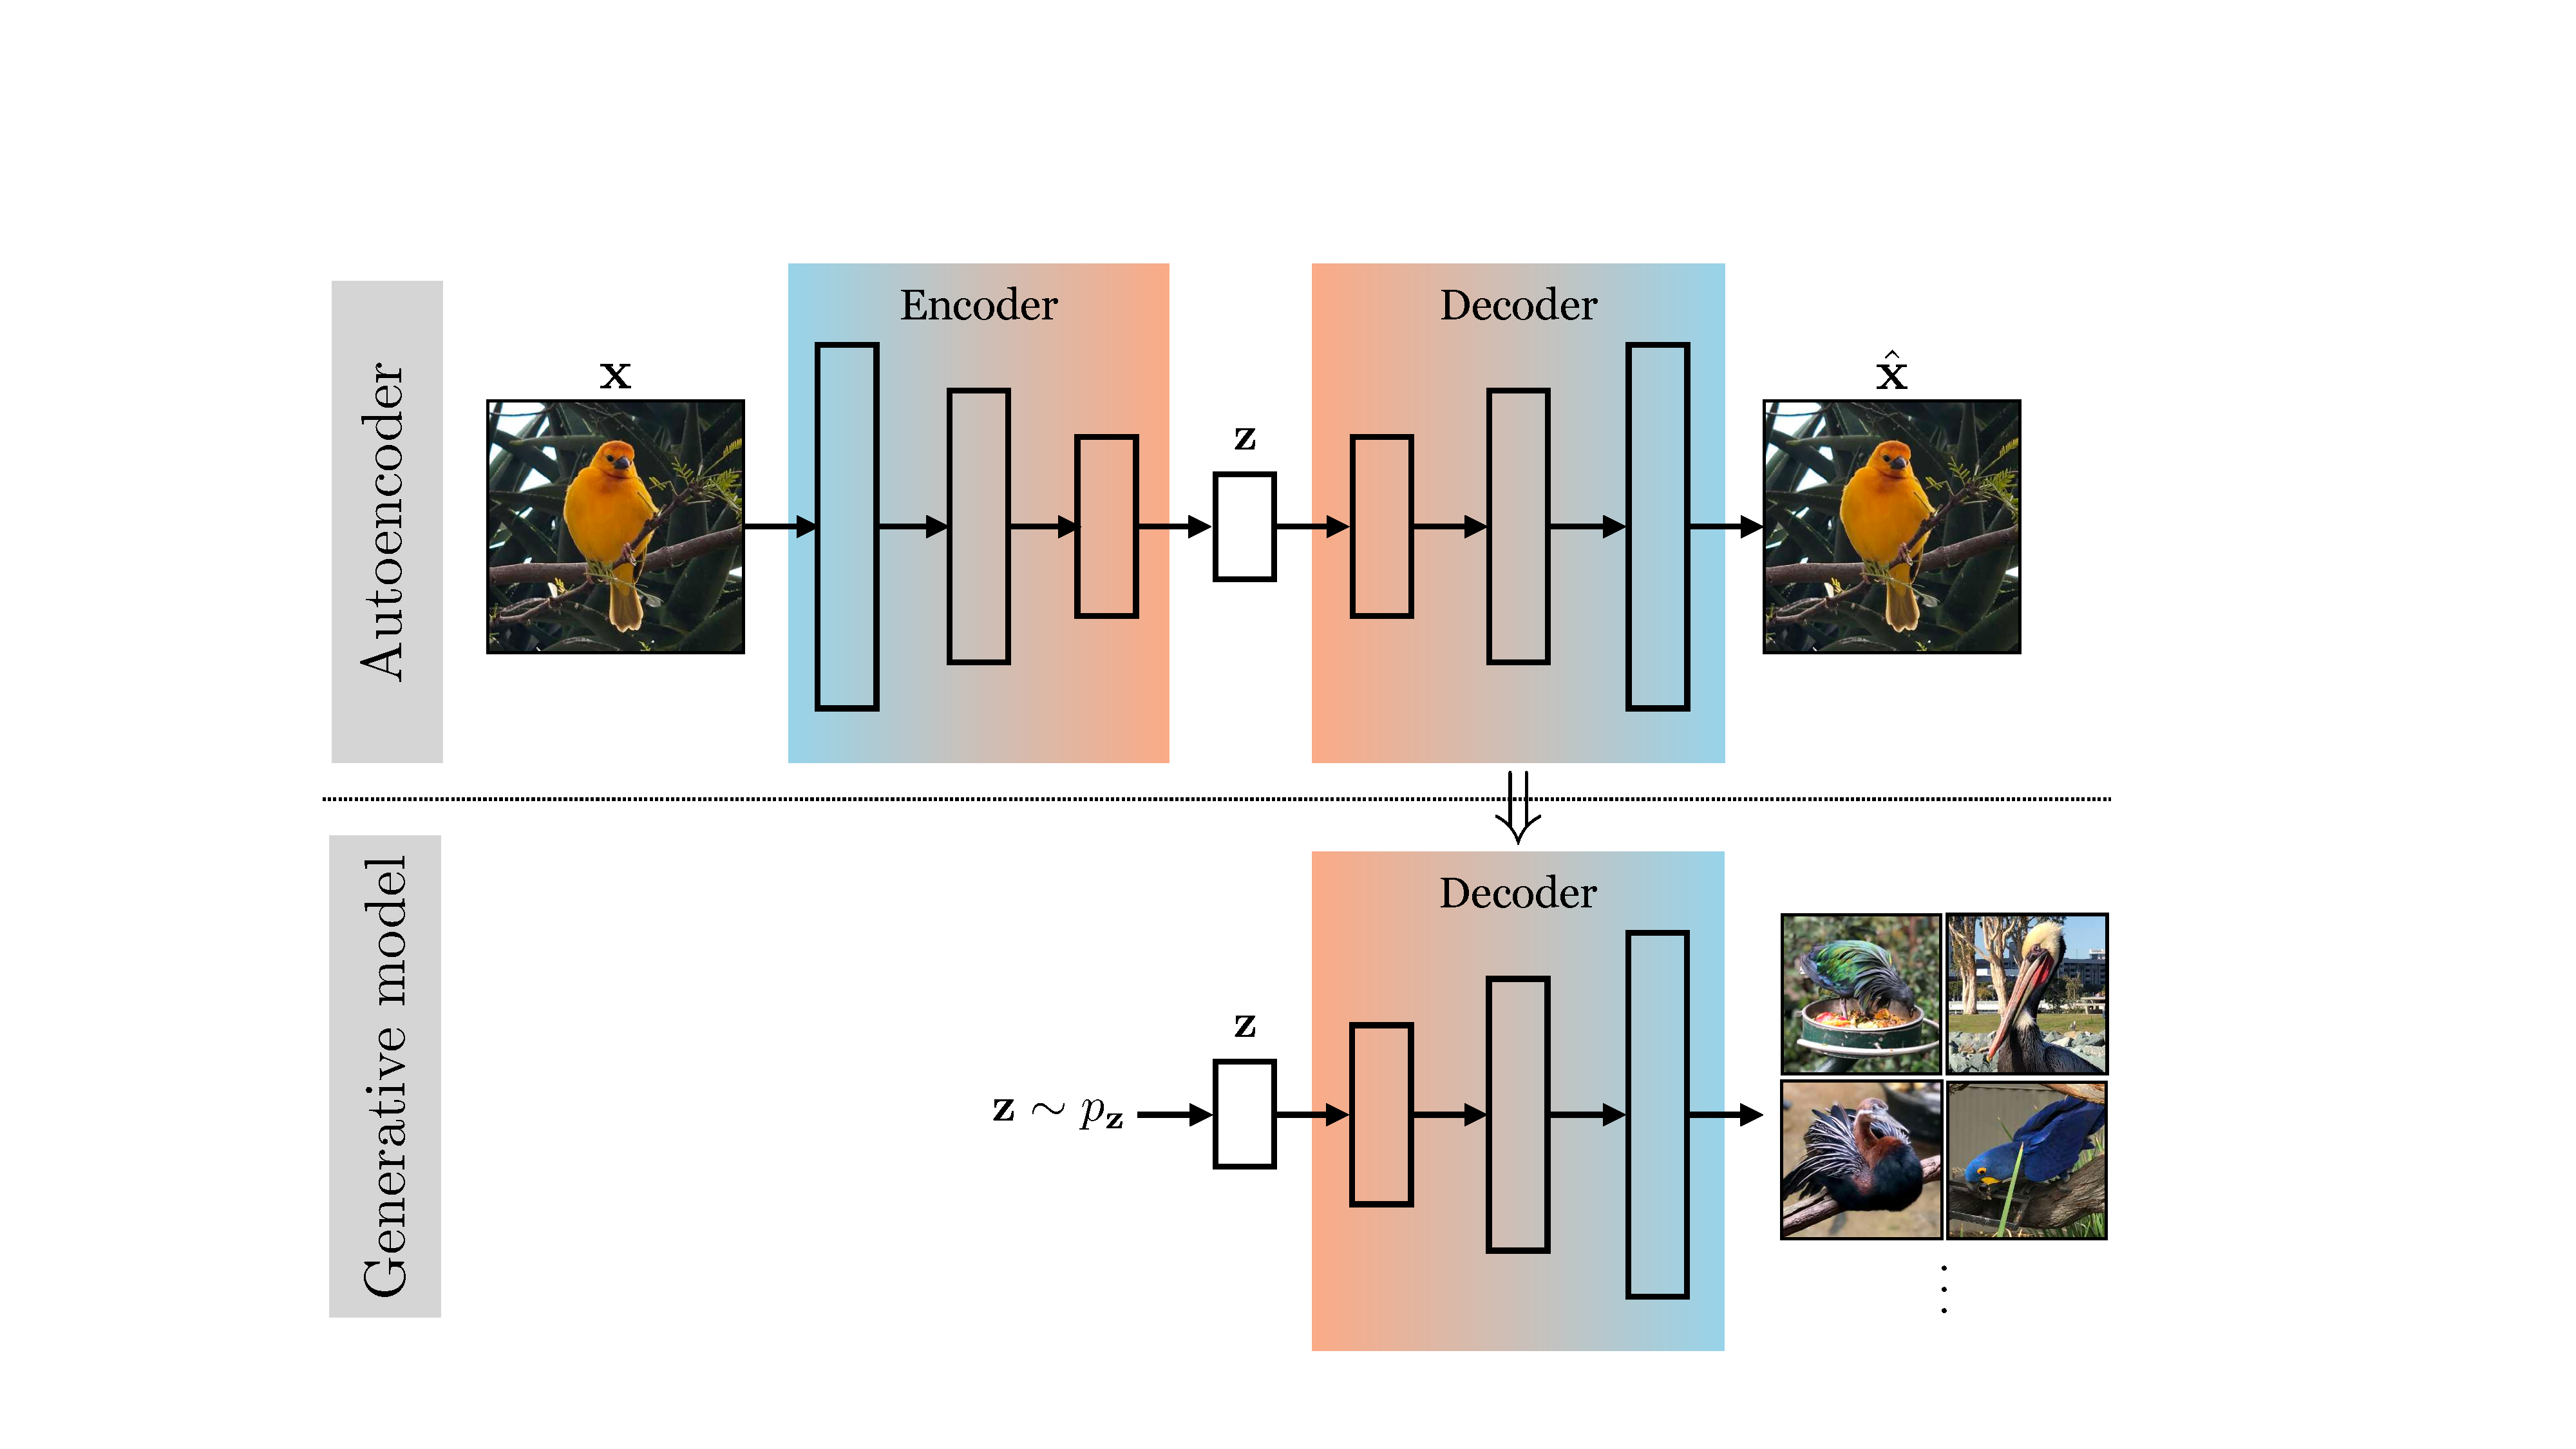
\includegraphics[width=0.8\linewidth]{./figures/generative_modeling_and_representation_learning/autoencoder_to_generative_model.pdf}
    \label{fig:generative_modeling_and_representation_learning:autoencoder_to_generative_model}
\end{figure}

But how do we get this $\mathbf{z}$? One goal of generative modeling is to be able to make up random images from scratch. So we need a distribution from which we can sample $\mathbf{z}$'s from scratch, we need $p_{\mathbf{z}}$. An autoencoder doesn't directly give us this. You might ask, what if, after training an autoencoder, you just sample a random $\mathbf{z}$, say from a unit Gaussian, and feed it through the decoder? The problem is that this sample might be very different from what the decoder was trained on. Maybe encoder has learned to map all images to embeddings far from the origin. Then a unit Gaussian $\mathbf{z}$ would be far out of distribution and the decoder's behavior could be arbitrary. %Sure we can get $\mathbf{z}$'s by encoding images as $F(\mathbf{x})$, but then we need a way to sample random images from scratch, and we are back where we started.
\newpage
In general, the embedding space of an autoencoder might be just as complicated to model as the data space we started with:%\marginnote{Due to various implicit biases, autoencoder embeddings may turn out to be simpler than the data they are trained on.}
\begin{figure}[h!]
    \centering
    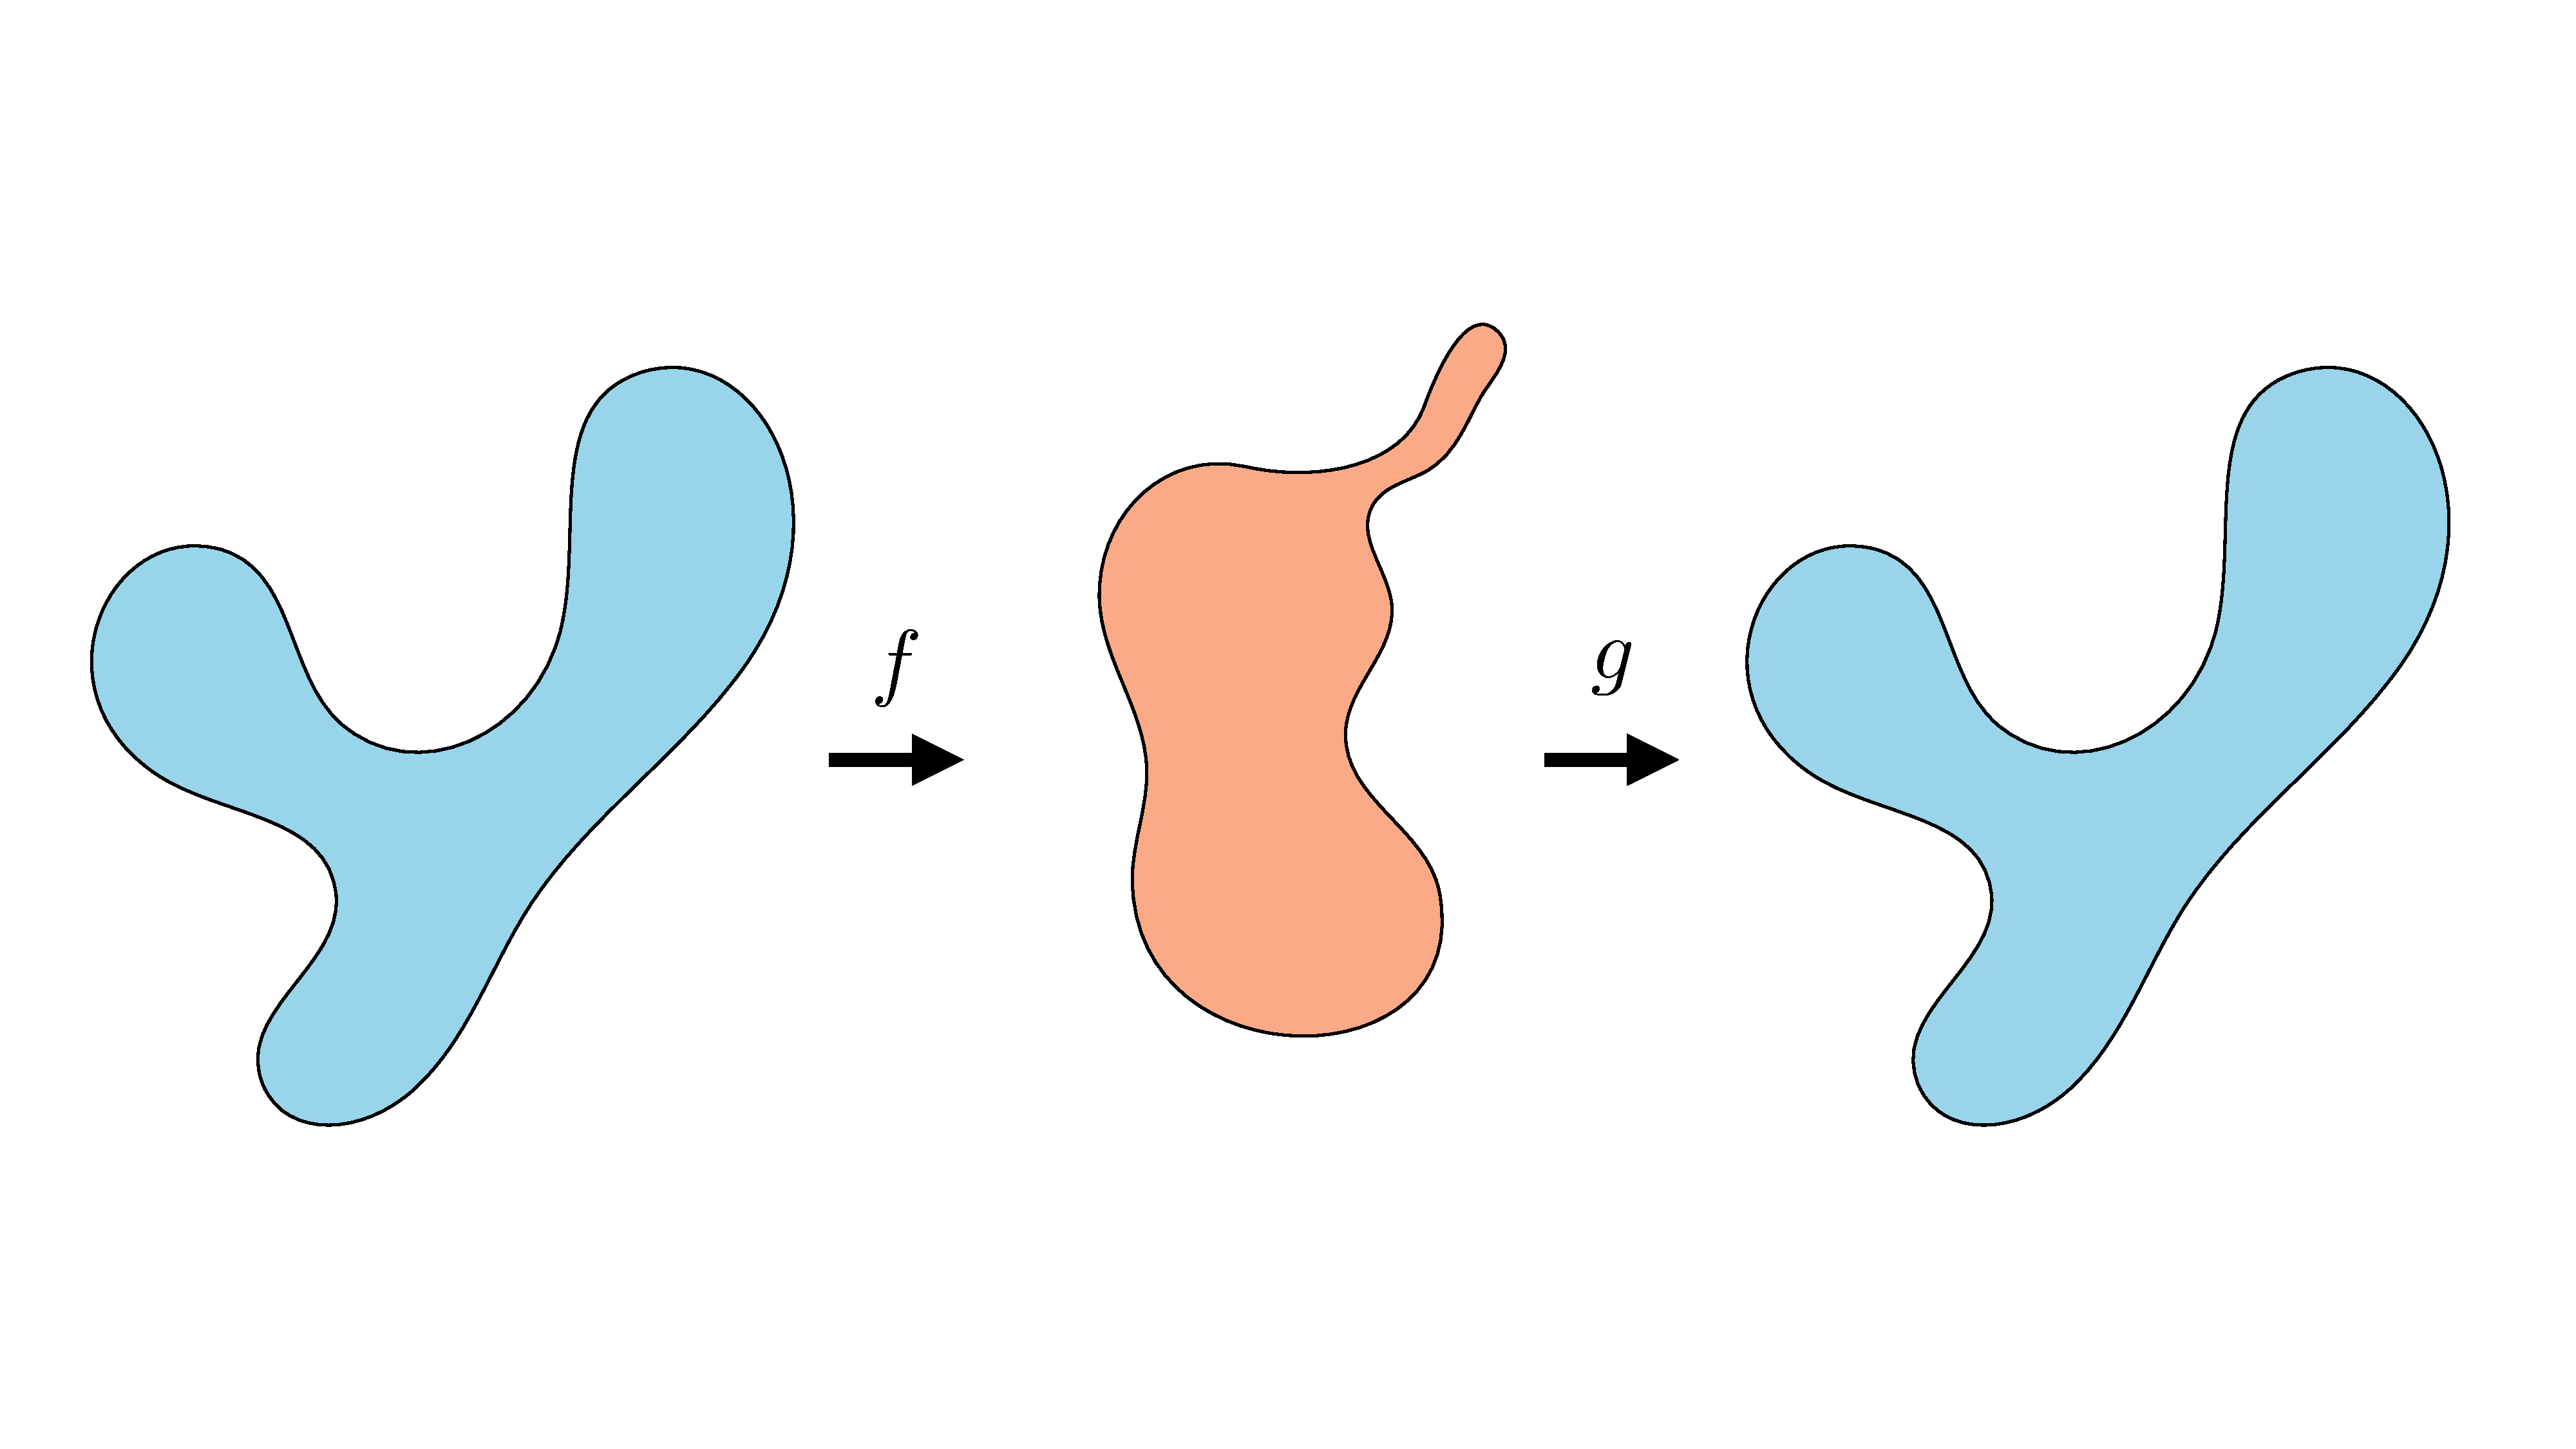
\includegraphics[width=0.6\linewidth]{./figures/generative_modeling_and_representation_learning/autoencoder_complicated_latent_space.pdf}
    \label{fig:generative_modeling_and_representation_learning:autoencoder_complicated_latent_space}
\end{figure}


\textbf{Variational autoencoders} (\textbf{VAE}s) are a way to turn an autoencoder into a proper generative model, which can be sampled from and which maximizes data likelihood under a formal probabilistic model. The trick is very simple: just take a vanilla autoencoder and 1) regularize the latent distribution to squish it into a Gaussian (or some other base distribution), 2) add noise to the output of the encoder. In code, it's essentially a two line change!

Okay, but seeing \textit{why} this is the right and proper thing to do requires quite a bit of math. We will derive it now, using a different approach than in most texts. We think this approach makes it more intuitive what is going on. See XX for the more standard derivation.

\subsection{The VAE likelihood model}

Mixture of Gaussians

\subsection{Optimizing VAEs -- the importance sampling trick}


\subsection{Do VAEs learn good representations?}



\section{Normalizing flows}

Next we will consider generative models with latent variables, $\mathbf{z}$. The models we will cover are implicit: they learn a generator which maps a base distribution over $\mathbf{z}$ to a transformed distribution over $\mathbf{x}$. Typically the base distribution is something simple like $p_{\mathbf{z}} = \mathcal{N}(0,1)$ and the mapping is a deep neural net. The difference between different methods is mainly in the learning objective, which encourages this mapping to fit the data distribution.

We will start with two implicit max likelihood models, normalizing flows and variational autoencoders. These models share the same objective as autoregressive models -- assign maximum probability density to the training datapoints -- but differ in how they achieve this. For max likelihood models, we need to calculate or approximate the data likelihood function, $L(\{\mathbf{x}^{(i)}\}_{i=1}^N, \theta)$, but how we calculate likelihood can be done in a few ways. In explicit density models, like autoregressive models, we directly learn the likelihood function: $L(\{\mathbf{x}^{(i)}\}_{i=1}^N, \theta) = \prod_i p_{\theta}(\mathbf{x}^{(i)})$. Then we adjust the parameters to maximize this quantity.

In implicit models, things are a bit harder since we don't have an explicit likelihood function. Instead we learn a generator $G_{\theta}$. If the sampler is bijective, so that $G^{-1}$ exists and can be computed, things are actually still easy. We can use the {\bf change of variables} formula to compute the likelihood of data implied by our sampler:
\begin{equation*}
    L(\mathbf{x}, \theta) = p_{\mathbf{z}}(G_{\theta}^{-1}(\mathbf{x}))|\det(\frac{\partial G_{\theta}^{-1}(\mathbf{x})}{\partial \mathbf{x}})| 
\end{equation*}
%where $p_{\mathbf{z}}$ is our prior (usually a Normal distribution or uniform distribution).

Max likelihood learning corresponds to maximizing the log likelihood of the training data, $\{\mathbf{x}^{(i)}\}_{i=1}^N$, so here it looks like:
\begin{equation}
    \argmax_{G_{\theta}} \frac{1}{N} \sum_{i=1}^N \log p_{\mathbf{z}}(G_{\theta}^{-1}(\mathbf{x}^{(i)})) + \log |\det(\frac{\partial G_{\theta}^{-1}(\mathbf{x}^{(i)})}{\partial \mathbf{x}^{(i)}})|\label{eqn:generative_models:normalization_flows}
\end{equation}
{\bf Normalizing flows} are generative models learned using Equation \ref{eqn:generative_models:normalization_flows}. The name is a reference to the fact that the generator is bijective (a ``flow") and the latent variables have a known (``normalized") density they are drawn from.

%{\bf Diffusion models} are a kind of normalizing flow. They define an invertible process that adds noise to an image in a series of steps. With enough steps, the image because completely random noise. Because each step is invertible, the process can be reversed: first sample random noise, then step by step ``congeal" it into an image. <-- this is wrong, diffusion models are not bijective


\section{Generative adversarial networks}



\subsection{Variational Autoencoders}

In Chapter \ref{chapter:representation_learning} we learned about autoencoders.

Notice that the second half of an autoencoder looks like a generator. It takes encodings z as input and produces images as outputs. So a natural thing to try is to just take a random z as input in order to produce a random image as output. Then it would act like a generative model. Unfortunately if we do that then it doesn't work because we don't know the distribution of latents and most don't map to natural looking images.

The Variational Audoencoder fixes this problem.



%A shortcoming of normalizing flows is that the latent variables have to be of the same dimensionality as the data. 

If the mapping is not bijective, the change of variables formula does not apply. Instead, one option is to build up a density model, from our sampler, by putting a little blip of Gaussian probability around each image, $G_{\theta}(\mathbf{z}^{(i)})$, generated by our sampler. Commonly, we augment $G$ to also output the variance, $\sigma$, of this Gaussian, so we have $G^{\mu}_{\theta}$ and $G^{\sigma}_{\theta}$. This gives us an infinite mixture of Gaussians as our likelihood model: $L(\mathbf{x}, \theta) = \int_{\mathbf{z}} p_{\theta}(\mathbf{x} | \mathbf{z})p(\mathbf{z})d\mathbf{z}$, where $p_{\theta}(\mathbf{x} | \mathbf{z}) = \mathcal{N}(\mathbf{x}; G_{\theta}^{\mu}, G_{\theta}^{\sigma})$ and $p_{\mathbf{z}}$ is usually a unit Normal distribution.

Find the distribution such that drawing one sample from that distribution will be as good as possible an estimate of the integral.

With a finite mixture, we can pick the component that dominates the sum and clearly this is a lower-bound on likelihood since we ignored the other terms in the sum.

But picking this component requires evaluating each component, so we have no savings! Instead we will try to \textit{predict} which component dominates the sum for each datapoint just by looking at the datapoint, so we have a prediction problem z* = argmax p(x|z)p(z). Remember, searching over all z gives no savings, so we will amortize it during training: E(x) = z*, which we can train with a classification loss: E = argmax xent(z*, E(x)). More generally, we can use a max likelihood loss q(z* | x). Or we can write it as argmax p(x|E(x))p(E(x)). Really we want q(z|x) to be as close as possible to the true, unknown distribution p(z|x).

But there's a problem: it's not differentiable, w.r.t. our probability model $p_\theta$, to zero-out all but the top component. We can make it differentiable by predicting a distribution over components. (A sample from this distribution lets us approximate the gradient since dE[x] = E[dx].)

Now clearly we can increase the number of mixture components toward infinity. In the continuous setting we need to define a distribution over the continuum (for differentiability) so let's use a Gaussian for simplicity. Also, as the number of components goes to infinity, they take on infinitesimal weight. So again we will have a bad estimate. Instead let's take a region of z space. If the region is as big as all of z space then a lot of samples are pointless. If it's too small then we are really underestimating the probability. So we want it to be not too large and not too small. We will use a Gaussian. Any sub-region of z space is fine, up to and including the entire space, because it will always be a lower-bound until we include the entire space.

Basically we are just taking a subpart of the full integral. We don't want that subpart to be too small or it's a bad approximation. Nor too big, since then sampling won't be efficient. We will choose a Gaussian shaped subpart. Why doesn't this overcount? Because it weighs intervals less than unity...


We want to approximate the integral E[dx], which gives us the gradient. We could take the expectation over p(z) of course, or do importance weighting. So I guess we will use importance sampling on that integral, with importance weights given by q(z|x). So then the task is to just learn q(z|x). And sure that involves another integral but we can also approximate that one by sampling, and that one can be approximated more efficiently since p(z|x) is a narrower distribtuion than p(z).


We can get a better estimate by predicting the top k components in the sum. One way to do so cheaply is predict a distribution over components and sample k items from it. This will still be a lower bound if we divide by k.

%In the general case, we have $L(\mathbf{x}, \theta) = \int_\mathbf{z} \mathbbm{1}(\mathbf{x} = G_{\theta}(\mathbf{z}))p(\mathbf{z})d\mathbf{z}$. This integral is intractable. We can use the calculus of variations to approximate it. Commonly, we add some noise to $G_{\theta}(\mathbf{z})$, which makes the formulas differentiable.% (we will see this more clearly in just a bit).

This integral is usually very expensive to compute so we will approximate it, and this leads to a method called {\bf Variational Autoencoders} ({\bf VAEs}). The first trick in VAEs is to use a \textit{Monte Carlo estimate} of the integral:
\begin{align}
    L(\mathbf{x}, \theta) &= \int_{\mathbf{z}} p_{\theta}(\mathbf{x} | \mathbf{z})p(\mathbf{z})d\mathbf{z} \label{eqn:generative_models:vae_likelihood}\\
    &= \mathbb{E}_{\mathbf{z}\sim p(\mathbf{z})}[p_{\theta}(\mathbf{x} | \mathbf{z})]\\
    &\approx \frac{1}{N} \sum_{i=1}^N p_{\theta}(\mathbf{x} | \mathbf{z}^{(i)}), \quad \mathbf{z}^{(i)} \sim p(\mathbf{z})
\end{align}
So far so good, but for this to be a good approximation our number of samples, $N$, may need to be very large. Now here comes the real trick: \textit{try to only sample those $\mathbf{z}$'s that are actually responsible generating the observed $\mathbf{x}$, i.e. those $\mathbf{z}$'s for which $p_{\theta}(\mathbf{x}, \mathbf{z})$ is large}. The idea is that for most $\mathbf{z}$'s, $p_{\theta}(\mathbf{x}, \mathbf{z})$ will end up being near zero. This idea is called {\bf importance sampling}. Rather than sampling $\mathbf{z}^{(i)} \sim p(\mathbf{z})$ to approximate the integral, we sample from another distribution $\mathbf{z}^{(i)} \sim q(\mathbf{z})$, and multiply by a correction factor $\frac{p(\mathbf{z})}{q(\mathbf{z})}$ to account for the fact that we are sampling from a biased distribution:
\begin{align}
L(\mathbf{x}, \theta) &= \mathbb{E}_{\mathbf{z}\sim p(\mathbf{z})}\Big[p_{\theta}(\mathbf{x} | \mathbf{z})\Big] \label{eqn:generative_models:vae_likelihood2}\\
&= \mathbb{E}_{\mathbf{z}\sim q(\mathbf{z})}\Big[\frac{p(\mathbf{z})}{q(\mathbf{z})} p_{\theta}(\mathbf{x} | \mathbf{z})\Big]%\\
&\approx \frac{1}{N} \sum_{i=1}^N \frac{p(\mathbf{z}^{(i)})}{q(\mathbf{z}^{(i)})} p_{\theta}(\mathbf{x} | \mathbf{z}^{(i)}), \quad \mathbf{z}^{(i)} \sim q(\mathbf{z})
\end{align}
As can be seen if you write out the integral, the two expectations above are \textit{exactly equal}, and this is true for \textit{any} distribution $q$. Intuitively, as we alluded to above, we want the samples from $q$ to be the dominate terms in the integral in Eqn. \ref{eqn:generative_models:vae_likelihood}, so that only a few samples will suffice to well approximate the integral. The theory of importance sampling tells us that indeed this is the optimal thing to do and in particular we should ideally set $q = p_{\theta}(\mathbf{z}|\mathbf{x})$, i.e. $q$ should be a prediction of exactly which $\mathbf{z}$ was responsible for generating the observed $\mathbf{x}$. 

Now we have a goal in mind for $q$: we want $q$ to be as close as possible to $p_{\theta}(\mathbf{z}|\mathbf{x})$. This way we will get the best estimate of the likelihood $L$ when we use that learned $q$. Note that since $q$ can be any distribution, it can, for instance, be a distribution conditioned on $\mathbf{x}$, and that's what we will use so as to best approximate $p_{\theta}(\mathbf{z}|\mathbf{x})$, since it is also conditioned on $\mathbf{x}$. Further, because we are learning parameters of a parametric distribution $q$, we will rewrite $q$ as $q_{\phi}$ to make explicit that $\phi$ are the parameters being learned. Given this notation, we can state our goal for $q$ as we want to minimize $\texttt{KL}(q_{\phi}(\mathbf{z}|\mathbf{x}), p_{\theta}(\mathbf{z}|\mathbf{x}))$.

Alas, evaluating this KL-divergence requires evaluating $p_{\theta}(\mathbf{z}|\mathbf{x})$, which yields another intractable integral. Fortunately, something rather magical happens when we do a few algebraic manipulations:
\begin{align}
    \texttt{KL}(q_{\phi}(\mathbf{z}|\mathbf{x}), p_{\theta}(\mathbf{z}|\mathbf{x})) &= \mathbb{E}_{q_{\phi}(\mathbf{z}|\mathbf{x})}[\log q_{\phi}(\mathbf{z}|\mathbf{x}) - \log p_{\theta}(\mathbf{z}|\mathbf{x})]\\
    &= \mathbb{E}_{q_{\phi}(\mathbf{z}|\mathbf{x})}[\log q_{\phi}(\mathbf{z}|\mathbf{x}) - \log p_{\theta}(\mathbf{z}, \mathbf{x})] + \log p_{\theta}(\mathbf{x})\\
    &= -\mathcal{L}(\mathbf{x}, \theta, \phi) + \log p_{\theta}(\mathbf{x})\\
    &= -\mathcal{L}(\mathbf{x}, \theta, \phi) + \log L(\mathbf{x}, \theta)\\
    \mathcal{L}(\mathbf{x}, \theta, \phi) &= \log p_{\theta}(\mathbf(x)) - \texttt{KL}(q_{\phi}(\mathbf{z}|\mathbf{x}), p_{\theta}(\mathbf{z}|\mathbf{x}))\\
    &\leq \log p_{\theta}(\mathbf(x))
\end{align}

Now $\mathcal{L}$ is something we can actually evaluate and therefore optimize over! Notice that $\mathcal{L}$ is a lower-bound on the log likelihood of the data (last line, because KL-divergence is always non-negative), and because of this $\mathcal{L}$ is referred to as the {\bf Evidence Lower-Bound} or {\bf ELBO}. Because $\mathcal{L}$ is a lower-bound, gradient ascent on $\mathcal{L}$, w.r.t. parameters $\theta$ and $\phi$ will produce a model $p_{\theta}$ that places maximum likelihood on the data. Interestingly, as $\mathcal{L}$ is being maximized, the gap between the $\mathcal{L}$ and $\log L$ will eventually have to decrease, as we approach the true max likelihood model in the family of functions we are optimizing over. That means that $\texttt{KL}(q_{\phi}(\mathbf{z}|\mathbf{x}), p_{\theta}(\mathbf{z}|\mathbf{x}))$ will have to decrease, since it equals the gap between $\mathcal{L}$ and $\log L$. Therefore something really neat has happened, we are getting better and better importance weights $q$ as the model $p$ also gets better and better, and the better the importance weights are, the better, in turn, is our ability to estimate likelihood from just a few samples. It turns out that in practice, one sample per $\mathbf{x}$ per step of gradient ascent is enough, because over the course of optimization this single sample becomes a better and better estimate of the likelihood we are trying to optimize.

A longer treatment on VAEs is given in \cite{doersch2016tutorial}.

%That means wiggling parameters to increase $\mathcal{L}$ will \textit{have to} 

%How should we measure the distance between $q_{\phi}$ and $p_{\theta}(\mathbf{z}|\mathbf{x})$? We will use the KL-divergence between the two distributions, i.e. $\texttt{KL}(q_{\phi}(\mathbf{z}|\mathbf{x}), p_{\theta}(\mathbf{z}|\mathbf{x}))$. Now we have two goals: 1) minimize this KL-divergence to get a good $q_{\phi}$ for importance sampling, and 2) maximize the data likelihood, using importance sampling to efficiently estimate it.

% In VAEs, rather than directly maximizing the likelihood function in Eqn. \ref{eqn:generative_models:vae_likelihood2}, we instead take the $\log$ of the term inside the expectation:
% \begin{align}
%     \mathcal{L}(\mathbf{x}, \theta) &= \mathbb{E}_{\mathbf{z}\sim p(\mathbf{z})}\Big[ \log p_{\theta}(\mathbf{x} | \mathbf{z})\Big]
% \end{align}
% By Jensen's inequality, this is a lower-bound on the data log likelihood ($\mathbb{E}[\log x] \leq \log \mathbb{E}[x]$). Hence under this transformation, we are maximizing a lower-bound on the data log likelihood. Now we can state the full VAE learning objective:
% \begin{align}
%     \argmin_{\theta,\phi} \texttt{KL}(q_{\phi}(\mathbf{z}|\mathbf{x}), p_{\theta}(\mathbf{z}|\mathbf{x})) + \mathcal{L}(\mathbf{x}, \theta)
% \end{align}

%The next question is then how to choose the best $q$ such that we can get a good approximation to the expectation with just a few samples?

%Here we can use the idea alluded to above, and try to sample $\mathbf{z}$'s such that $p_{\theta}(\mathbf{x} | \mathbf{z})$ is large. 

%We can set this up as an optimization problem. First, notice that:
%\begin{align}
%     \frac{1}{N} \sum_{i=1}^N \frac{p(\mathbf{z}_i)}{q(\mathbf{z}_i)} p_{\theta}(\mathbf{x} | \mathbf{z}_i), \quad \mathbf{z}_i \sim q(\mathbf{z}) < \mathbb{E}_{\mathbf{z}\sim p(\mathbf{z})}[p_{\theta}(\mathbf{x} | \mathbf{z})]
% \end{align}
% for any probability distribution $q$. This is because 

%{\bf Variational Autoencoders} ({\bf VAEs}) are one popular way to use importance sampling to approximate an infinite mixture model likelihood function. Originally they were motivated by the idea of variational inference, but we will go with the importance sampling view, since we feel it makes VAEs much simpler to understand.

%The goal of the VAE is to approximate the likelihood function $L(\mathbf{x}, \theta)$.


%\textit{approximate the integral via well-chosen samples from $p(\mathbf{z})$}. 

%we turn to the calculus of variations of approximate it. The calculus of variations deals with finding functions that maximize some functional. A functional is just a function of functions. Here, the functional we have is an integral and the function is a probability density: we are trying to find a probability density that maximizes an integral. That's really all that is meant by the fancy word ``variational calculus" -- why do we need a special name for this? We don't, for our present purposes, but it's a term you are likely to encounter so it's good to remember it. 

%Saying we are using ``variational inference" usually just means we are using a tractable density $q$ to approximate an intractable target density $p$.

%Here is how it works in {\bf Variational Autoencoders} ({\bf VAEs}). We want to approximate $p(\mathbf{x}) = \int_\mathbf{z} p_{\theta}(\mathbf{x} | \mathbf{z})p(\mathbf{z})d\mathbf{z}$ in a tractable manner. We use $\int_\mathbf{z} p_{\theta}(\mathbf{x} | \mathbf{z})p(\mathbf{z})d\mathbf{z} \approx \int_\mathbf{z} p_{\theta}(\mathbf{x} | \mathbf{z})q_{\phi}(\mathbf{z}|\mathbf{x})d\mathbf{z}$, for some well chosen $q_{\phi}$. Which $q_{\phi}$ should we use? We'd like a $q_{\phi}$ such that $q_{\phi}(\mathbf{z}|\mathbf{x})$ places high density on exactly those $\mathbf{z}$'s that have high $p_{\theta}(\mathbf{x}|\mathbf{z})$. Then a few samples from $q$ will suffice to be a good approximation to the full integral. We can jointly learn $q_{\phi}$ and $p_{\theta}$ to achieve this. A fuller treatment of how VAEs achieve this goal is given in \cite{doersch2016tutorial}.

%Other popular deep generative models include {\bf Generative adversarial networks}, {\bf Autoregressive models}, and {\bf Energy-based models}.

%In this case, the mapping either folds or tears the, or both. If it tears, then there are some $\mathbf{x}$'s that $g(z)$ cannot produce. To fill in the gaps, we can use the trick $\mathbf{x} = g(\mathbf{z}) + \epsilon$. This places non-zero density on all of $\mathbf{x}$.


%\subsection{Variational autoencoder}
%Variational autoencoders (VAEs) are infinite mixture models. A mixture model approximates a density by a sum of simple distributions. VAEs typically use an infinite sum of Gaussians. This infinite mixture can be described by an infinite number of means and variances of each Gaussian. How can we represent an infinite set of parameters with a finite number of parameters? The VAE's approach is to parameterize the 

\subsection{Generative adversarial networks}

{\bf Generative adversarial networks}, or {\bf GANs}, are another kind of implicit generative model, introduced in \cite{goodfellow2014generative}. Unlike VAEs, GANs do not require an encoder and in their vanilla form, only involve a decoder, which is also called a {\bf generator}, $G$. GANs learn a mapping $G: \mathcal{Z} \rightarrow \mathcal{X}$ such that the generated outputs are \textit{indistinguishable from real images}, $\mathbf{x} \in \mathcal{X}$, according to a {\bf discriminator} network $D$. $G$ and $D$ play an adversarial game in which $G$ tries to become better and better at generating fake images while $D$ tries to become better and better at detecting fakes. The learning problem can be written as a minimax game:
\begin{align}
    \argmin_G\max_D \mathbb{E}_{\mathbf{x} \sim p_{\texttt{data}}}[\log D(\mathbf{x})] + \mathbb{E}_{\mathbf{z} \sim p_{\mathbf{z}}}[\log (1-D(G(\mathbf{z})))]\label{eqn:generative_models:GAN_learning_problem}
\end{align}
This objective may be easier to understand if we think of the objectives for $G$ and $D$ separately. Given a particular generator $G$, $D$ tries to maximize its ability to discriminate between real and fake images (fake images are anything output by $G$). $D$'s objective is logistic regression between a set of real data $\{\mathbf{x}^{(i)}\}_{i=1}^N$ and fake data $\{\mathbf{x}^{(i)}\}_{i=1}^N$, where $\hat{\mathbf{x}}^{(i)} = G(\mathbf{z}^{(i)})$.

Let the optimal discriminator be labeled $D^*$. We have that:
\begin{align}
    D^* = \argmax_D \mathbb{E}_{\mathbf{x} \sim p_{\texttt{data}}}[\log D(\mathbf{x})] + \mathbb{E}_{\mathbf{z} \sim p_{\mathbf{z}}}[\log (1-D(G(\mathbf{z})))] \label{eqn:generative_models:GAN_optimal_D}
\end{align}

Now we turn to $G$'s perspective. Given $D^*$, $G$ tries to solve the following problem:
\begin{align}
    \argmin_G \mathbb{E}_{\mathbf{z} \sim p_{\mathbf{z}}}[\log (1-D^*(G(\mathbf{z})))] \label{eqn:generative_models:GAN_optimal_G}
\end{align}

Now, because the optimal discriminator $D^*$ depends on the current behavior of $G$, as soon as we \textit{change} $G$, updating it to better fool $D^*$, $D^*$ no longer is the optimal discriminator and we need to again solve problem in Eqn. \ref{eqn:generative_models:GAN_optimal_D}. To optimize a GAN, we simply alternate between taking one gradient on Eqn. \ref{eqn:generative_models:GAN_optimal_G} and then $K$ gradient steps on Eqn. \ref{eqn:generative_models:GAN_optimal_D}, where the larger the $K$, the closer we are to approximating the true $D^*$. In practice, setting $K=1$ is often sufficient.

\paragraph{GANs are statistical image models}
GANs are related to the statistical image models we saw in Chapter XX. In Heeger \& Bergen, for example, we synthesize images with the same statistics as a source texture. This can be phrased as an optimization problem in which we optimize image pixels until certain statistics of the images match those same statistics measured on a source (training) set of images. We can write it as $\norm{\phi(x) - \phi(\hat{x})}$. This is a kind of discriminator -- it outputs a score related to the difference between a generated image and real data. However, unlike a GAN, this discriminator is hand-defined in terms of certain statistics of interest rather than learned. Additionally, GANs amortize the optimization over pixels that satisfy the ``discriminator". That is GANs learned a mapping $G$ from latent noise to samples rather than arriving at samples via an optimization process that starts from scratch each time we want to make a new sample.


\subsection{Deep energy-based models}
One way to think about the discriminator in GANs is as an {\bf energy function} that we want to minimize. While in GANs this energy function changes to penalize whatever current errors the generator is making, would it be possible to learn a ``universal" discriminator that will properly score any type of real or fake imagery and doesn't have to be updated when $G$ changes? This is the idea of {\bf energy-based models}, or {\bf EBMs}.

With energy-based model, the emphasis is on the energy function, $E$, rather than on the generator -- in fact, there usually is not generator. Instead we can use Markov Chain Monte Carlo (MCMC) to sample from $E$. The energy function is an unnormalized probability distribution, i.e. it is a function $E: \mathcal{X} \rightarrow \mathbb{R}$. We can parameterize $E$ as a neural net -- it's just a net that takes an image as input and produces a real-valued scalar as output.

MCMC is a method for producing samples from an unnormalized probability distribution, and that's how you sample from an EBM. How do you learn an EBM? First, we definitely want to assign low energy (that is, high probability) to the training datapoints; the first part of the objective of an EBM is to maximize $E(\mathbf{x})$ when $\mathbf{x} \sim p_{data}$. Now, to prevent the energy to go to zero \textit{everywhere} we also need a negative term that will increase energy where there are no datapoints. One option is to just randomly sample ``noise" and increase the energy on this noise. But we can be much more efficient by increasing the energy on ``hard negatives" which are fake images sampled from the current energy function. In particular, it turns out that the gradient of the likelihood function corresponding to an energy-based model has a form that can be evaluated \textit{without normalizing the energies} just by calculating the difference between the energy assigned to real and fake sampled images [XX Turner 2005]:
\begin{align}
    \nabla_{\theta}L(\{\mathbf{x}^{(i)}\}_{i=1}^N, \theta) \approx \mathbb{E}_{\mathbf{x} \sim p_{\texttt{data}}}[\nabla_{\theta}E_{\theta(\mathbf{x})}] - \mathbb{E}_{\mathbf{x} \sim p_{E}}[\nabla_{\theta}E_{\theta(\mathbf{x})}]
\end{align}
where $p_{E}$ is the normalized energy function $E_{\theta}/Z$; note again that we do not need to compute $Z$ but can still draw samples from $p_{E}$ using MCMC.

Notice that this objective is very similar to that of a GAN, except:
\begin{enumerate}
    \item GANs learn a generator $G$ rather than using MCMC as a sampler that implicitly draws samples from $\frac{E}{Z}$.
    %\item The GAN discriminator models the \textit{gradient} of an energy function, rather than the energy function itself. Therefore $D$, unlike $E$ cannot be directly used to estimate (unnormalized) likelihoods. 
    \item The GAN generator is where a lot of the magic of GANs occurs: it is a mapping from low-dimensional latent variables to images. The latent variables turn out to be a remarkably powerful representation of images, with numerous downstream applications. EBMs don't have these latent variables.
\end{enumerate}

